\documentclass[
    a4paper, aps, twocolumn, floatfix, superscriptaddress,
    nofootinbib]{revtex4-1}

% It's nice to be able to write your own name
\usepackage[T1]{fontenc}
% Automatic clickable links
\usepackage{hyperref}
% SI-units
\usepackage{siunitx}
% Enhanced math formatting
\usepackage{amsmath}
% Extended math symbols
\usepackage{amssymb}
% Include proof environment
\usepackage{amsthm}
\usepackage{enumerate}
% Import the tensor package for tensors
\usepackage{tensor}
% Include dod and dpd fracs
\usepackage{commath}
% Include font for the identity operator
\usepackage{dsfont}
% Include Tikz
\usepackage{tikz}
% Tikz add-on
\usetikzlibrary{shapes,arrows}
\usetikzlibrary{positioning}
% Several figures in the same figure
\usepackage{subfig}
% Appendix
\usepackage[toc, page]{appendix}
\usepackage{simpler-wick}
% Code listings
\usepackage{listings, lstautogobble}
\usepackage{minted}
% Colors
\usepackage{xcolor}
% Directory tree package
\usepackage{dirtree, varwidth}
% Multirow (for table)
\usepackage{multirow}

\usepackage{fontspec}
\newfontfamily\DejaSans{DejaVu Sans}

\newcommand{\nan}{\DejaSans 😱}

% Macro for latin-letter vectors
\newcommand{\vf}{\mathbf}
% Macro for greek-letter vectors
\newcommand{\vfg}{\boldsymbol}

% Fast macro for real-numbers R
\newcommand{\R}{\mathbb{R}}
% Fast macro for complex-numbers C
\newcommand{\C}{\mathbb{C}}
% Fast macro for polynomial room P
\renewcommand{\P}{\mathbb{P}}
% New command for the identity operator
\newcommand{\1}{\mathds{1}}
% New command for the Lagrangian density
\newcommand{\cL}{\mathcal{L}}
% New command for the Hamiltonian density
\newcommand{\cH}{\mathcal{H}}
% Fast macro for partial differential tensors
\newcommand{\tpl}[1]{\tensor{\partial}{_#1}} % Lower
\newcommand{\tpu}[1]{\tensor{\partial}{^#1}} % Upper
% Fast macro for tensors
\newcommand{\te}[1]{\tensor{#1}}
% Fast macro for commutation and anti-commutation relations
\newcommand{\com}[2]{\left[#1, #2\right]}
\newcommand{\acom}[2]{\left\{#1, #2\right\}}

% Macros for writing auto-sized paranthesis, brackets and braces
\newcommand{\para}[1]{\left(#1\right)}
\newcommand{\brak}[1]{\left[#1\right]}
\newcommand{\brac}[1]{\left\{#1\right\}}

% Macro for creating orbital bra-ket's, i.e., bra-ket with paranthesis edges
\newcommand{\obra}[1]{( #1 \lvert}
\newcommand{\oket}[1]{\rvert #1 )}
\newcommand{\obraket}[2]{( #1 \lvert #2 )}

% Macro for expectation value
\newcommand{\expv}[1]{\langle #1 \rangle}

\newcommand{\half}{\frac{1}{2}}

\newcommand{\bra}[1]{\langle #1\lvert}
\newcommand{\ket}[1]{\rvert #1\rangle}
\newcommand{\braket}[2]{\langle #1 \vert #2 \rangle}

\newcommand{\acr}[1]{a_{#1}^{\dagger}}
\newcommand{\ade}[1]{a_{#1}}

\newcommand{\kslat}{\ket{\Phi_0}}
\newcommand{\bslat}{\bra{\Phi_0}}

\newcommand{\kcc}{\ket{\Psi_{\text{CC}}}}
\newcommand{\bcc}{\bra{\Psi_{\text{CC}}}}

\newcommand{\ecc}{E_{\text{CC}}}
\newcommand{\eccd}{E_{\text{CCD}}}

% Defining color
\definecolor{light-gray}{gray}{0.9}

% Bash language specifier
\lstnewenvironment{bash}
{\lstset{
    basicstyle=\small\ttfamily, language=bash, keywordstyle=\color{blue},
    backgroundcolor=\color{light-gray}, showstringspaces=false,
    frame=single, autogobble=true, morekeywords={make, git},
    alsoletter={.}}}
{}

\begin{document}

\title{Ground state energy of quantum dots using the coupled cluster method}
\author{Winther-Larsen, Sebastian Gregorius}
\homepage[Project code: ]{https://github.com/Schoyen/FYS4411}
\affiliation{University of Oslo}
\author{Schøyen, Øyvind Sigmundson}
\homepage[Project code: ]{https://github.com/Schoyen/FYS4411}
\affiliation{University of Oslo}
\date{\today}

\begin{abstract}
    Something about coupled-cluster... Preferably doubles.
\end{abstract}

\maketitle
\tableofcontents

% FIXME: Replace the two-body matrix elements in bra-ket notation with u-tensor.

\section{Introduction}
    %TODO: Add explanation on why the many-body problem becomes intractable.
    % This can be shown by demonstrating that the true wavefunction of the system
    % must be a linear combination of all possible Slater detemerminants built up
    % from permutations of the single particle functions in the basis. Thus the
    % energy equation becomes too large.
    In this project we will study the ground state energy of quantum dots.

\section{Theory}
    In this project we will study a system of $N$ interacting electrons. We will
    be looking at a Hamiltonian consisting of a one-body and a two-body part.
    The one-body part is given by
    \begin{align}
        h(\vf{r}_i)
        &= -\half\nabla_i^2 + \half\omega^2 \vf{r}_i^2,
    \end{align}
    where we use natural units $\hbar = c = e = 1$ and set the mass to unity.
    % Why not write $\hbar = c = e = m = 1$?
    The two-body part is the Coulomb interaction potential.
    \begin{align}
        u(\vf{r}_i, \vf{r}_j)
        &= \frac{1}{\abs{\vf{r}_i - \vf{r}_j}}.
    \end{align}
    We thus get the total Hamiltonian
    \begin{align}
        H &= h + u
        =
        \sum_{i = 1}^N h(\vf{r}_i) + \sum_{i < j}^N u(\vf{r}_i, \vf{r}_j),
    \end{align}
    where $h$ is the full one-body operator and $u$ the full two-body
    operator, i.e., over the entire system.  Working in a basis of $L$ single
    particle functions, $\{\ket{p}\}_{p = 1}^L$. We define the reference Slater
    determinant as
    \begin{align}
        \ket{\Phi_0} &\equiv \ket{1, 2, \dots, N},
    \end{align}
    i.e., a tensorproduct of the $N$ first single particle functions, $\ket{i}$,
    of the system. We call these single particle functions \emph{occupied} as
    they are contained in the Slater determinant.  We will denote the occupied
    indices with $i, j, k, l, \dots \in \{1, \dots, N\}$, the \emph{virtual}
    states with $a, b, c, d, \dots \in \{N + 1, \dots, L\}$ and general indices
    with $p, q, r, s, \dots \in \{1, \dots, L\}$. In terms of sets of basis
    functions we can write this as
    \begin{align}
        \{\ket{p}\}_{p = 1}^L
        = \{\ket{i}\}_{i = 1}^N
        \cup
        \{\ket{a}\}_{a = N + 1}^L,
    \end{align}
    i.e., the general indexed states consists of both occupied and virtual
    states. Note that the single particle functions are orthonormal, i.e.,
    \begin{align}
        \braket{p}{q} = \delta_{pq}.
    \end{align}
    We can construct other Slater determinants in this basis by exciting
    or relaxing the reference determinant. A general excitation is labeled
    $\ket{\Phi_{ij\dots}^{ab\dots}}$ which means that we have removed the single
    particle functions with indices $i, j, \dots$ from the reference and added
    $a, b, \dots$. Note that
    \begin{align}
        \braket{\Phi^{ab\dots}_{ij\dots}}{\Phi_0} = 0,
        \label{eq:excited_overlap}
    \end{align}
    for any excitation.

    \subsection{Second quantization}
        Employing the creation operators, $\acr{p}$, and the destruction
        operators, $\ade{p}$, we can write the Hamiltonian as
        \begin{align}
            H
            &=
            \sum_{pq}h_{q}^{p}\acr{p}\ade{q}
            + \frac{1}{4}\sum_{pqrs}\bra{pq}\ket{rs}\acr{p}\acr{q}\ade{s}\ade{r},
        \end{align}
        where the sums are general indices over all $L$ basis states and the
        matrix elements are defined as
        \begin{gather}
            h^{p}_{q} \equiv \bra{p}h\ket{q}, \\
            \bra{pq}\ket{rs} \equiv \bra{pq}u\ket{rs} - \bra{pq}u\ket{sr}.
        \end{gather}
        Note that we use the chemists notation to label the antisymmetric matrix
        elements.

    \subsection{The coupled cluster approximation}
        We approximate the true wavefunction, $\ket{\Psi}$, of the system by the
        coupled cluster wavefunction, $\ket{\Psi_{\text{CC}}}$, defined by
        \begin{align}
            \ket{\Psi_{\text{CC}}}
            &\equiv e^{T}\ket{\Phi_0}
            = \para{
                \sum_{i = 0}^n
                \frac{1}{n!}T^n
            }\ket{\Phi_0},
        \end{align}
        where the \emph{cluster operator}, $T$, is given by a sum of
        $p$-excitation operators labeled $T_p$. They consist of \emph{cluster
        amplitudes}, $t_{i\dots}^{a\dots}$, and creation and annihilation
        operators.
        \begin{align}
            T &= T_1 + T_2 + \dots + T_p \\
            &=
            \sum_{ia}t_i^a\acr{a}\ade{i}
            + \para{\frac{1}{2!}}^2\sum_{ijab}
            t_{ij}^{ab}\acr{a}\acr{b}\ade{i}\ade{j}
            + \dots.
        \end{align}
        In the doubles approximation we limit the cluster operator to
        \begin{align}
            T \equiv T_2
            = \frac{1}{4}\sum_{ijab}t_{ij}^{ab}\acr{a}\acr{b}\ade{j}\ade{i}.
            \label{eq:T_2}
        \end{align}
        The first part of the coupled cluster method consists of constructing
        the cluster amplitudes using the \emph{amplitude equations}. After we
        have found the amplitudes we can compute the energy.

    \subsection{Energy of the coupled cluster approximation}
        When we're going to compute the energy of a system using the coupled
        cluster approximation we would ideally want to find the expectation
        value of the energy using the coupled cluster wavefunction.
        \begin{align}
            \ecc = \bcc H\kcc.
        \end{align}
        As it turns out, this is an uncomfortable way of finding the energy
        as $T \neq T^{\dagger}$. Instead we will define what we call the
        \emph{similarity transformed Hamiltonian}. We plug the coupled
        cluster wavefunction into the Schrödinger equation.
        \begin{align}
            H\kcc = \ecc\kcc.
        \end{align}
        Next, we left multiply with the inverse of the cluster expansion,
        i.e.,
        \begin{align}
            e^{-T}H\kcc = e^{-T}\ecc\kcc
            = \ecc \kslat.
            \label{eq:clean_schrodinger}
        \end{align}
        Projecting this equation on the reference state we get
        \begin{align}
            \ecc = \bslat e^{-T}H\kcc
            = \bslat e^{-T}He^{T}\kslat,
        \end{align}
        where in the latter inner-product we have located the similarity
        transformed Hamiltonian defined by
        \begin{align}
            \bar{H} \equiv e^{-T}He^{T}.
            \label{eq:similarity_transformed_hamiltonian}
        \end{align}

        To simplify the energy equation and the amplitude equations we use the
        normal ordered Hamiltonian.
        \begin{align}
            H = H_N + \bslat H\kslat.
        \end{align}
        The energy equation thus becomes
        \begin{align}
            \ecc &= \bslat\bar{H}\kslat
            = E_0 + \bslat e^{-T}H_N e^T\kslat,
        \end{align}
        where the reference energy is given by
        \begin{align}
            E_0 = \bslat H\kslat.
        \end{align}
        We now define the normal ordered similiarity transformed Hamiltonian as
        \begin{align}
            \bar{H}_N \equiv e^{-T}H_N e^T.
        \end{align}
        By expanding the exponentials of this Hamiltonian and recognizing the
        commutators we get the Baker-Campbell-Hausdorff expansion.
        \begin{align}
            \bar{H}_N
            &=
            H_N + \com{H_N}{T} + \frac{1}{2!}\com{\com{H_N}{T}}{T} + \dots.
        \end{align}
        From the connected cluster theorem we know that the only nonzero terms
        in the Baker-Campbell-Hausdorff expansion will be the terms where the
        normal ordered Hamiltonian has at least one contraction\footnote{In the
        Wick's theorem sense.} with every cluster operator on its right. This
        lets us write the expansion as
        \begin{align}
            \bar{H}_N
            &=
            H_N + \para{H_N T}_c + \frac{1}{2!}\para{H_N T^2}_c + \dots,
            \label{eq:sim_norm_hamiltionian_expansion}
        \end{align}
        where the subscript $c$ signifies that only contributions where at least
        one contraction between $H_N$ and $T$ has been performed will be
        included.

        \subsubsection{Coupled cluster doubles energy equation}
            Using the doubles approximation with the cluster operator $T_2$
            defined in \autoref{eq:T_2} the energy equation becomes
            \begin{align}
                \eccd
                &=
                E_0
                + \bslat e^{-T_2}H_N e^{T_2}\kslat.
            \end{align}
            As the doubles cluster operator doubly excites the reference and
            using the expansion in \autoref{eq:sim_norm_hamiltionian_expansion}
            we see that we can write the energy equation as
            \begin{align}
                \eccd
                &=
                E_0
                + \bslat H_N \kslat + \bslat (H_N T_2)_c\kslat,
            \end{align}
            as the Hamiltonian is only able to relax one pair of single
            particle functions. By construction we have that
            \begin{align}
                \bslat H_N \kslat = 0.
            \end{align}
            In the second term only the normal ordered two-body operator can
            contribute as the cluster operator gives a total excitation of $+2$.
            As we are projecting onto the reference we have to relax to zero
            again. The normal ordered Fock operator is at most able to excite
            and relax by $1$ and does therefore not contribute to the
            overall expression.
            \begin{align}
                \bslat (W_N T_2)_c \kslat
                &= \frac{1}{4}\sum_{ijab}\bra{ij}\ket{ab}t_{ij}^{ab}.
            \end{align}
            In total the energy equation reduces to
            \begin{align}
                \eccd
                &= \sum_{i} h_i^i + \half \sum_{ij}\bra{ij}\ket{ij}
                + \frac{1}{4}\sum_{ijab}\bra{ij}\ket{ab}t_{ij}^{ab},
            \end{align}
            where the first two terms come from the reference energy as shown in
            \autoref{eq:reference_energy}.

    \subsection{Coupled cluster amplitude equations}
        In order for us to solve the energy equation using the coupled cluster
        approximation we need to figure out what the cluster amplitudes,
        $t_{ij\dots}^{ab\dots}$, are. This is done by projecting
        \autoref{eq:clean_schrodinger} onto an excited Slater determinant, i.e.,
        \begin{align}
            \bra{\Phi_{ij\dots}^{ab\dots}}e^{-T}He^{T}\kslat
            = 0.
        \end{align}
        Note that in the amplitude equations we can use both the regular and the
        normal ordered Hamiltonian. They are equal as the reference energy term
        disappears due to \autoref{eq:excited_overlap}. The order of the
        excitation in the projection determines the order of the amplitudes you
        will find. In our case we are only interested in the second order
        ampltiudes found in the doubles approximation, hence we will solve the
        equation
        \begin{align}
            \bra{\Phi_{ij}^{ab}}e^{-T}H_N e^{T}\kslat = 0,
            \label{eq:doubles_amplitude_1}
        \end{align}
        to find an expression that can be used to solve for $t_{ij}^{ab}$.
        By employing the Baker-Campbell-Haussdorf (BCH) expansion,
        while setting $T= T_2$, we find
        \begin{equation}
                \bar{H}
                    = \Big(
                            H_N + H_NT_2
                            + \frac{1}{2}H_NT_2^2 \Big)_C.
        \label{eq:normal_order_expansion}
        \end{equation}
        The subscript $c$ indicates that only those terms in which the
        Hamiltonian is connected\footnote{In a Wick's theorem sense}
        to every cluster operator on its right should be included. Since
        the Hamiltonian contains at most four annihilation and creation
        operators, $H_N$ can connect to at most four cluster operators
        at once. Therefor, the BCH expansion must truncate at the
        fourth-order terms.

        Now comes the rather tedious task of evaluating all the terms
        that arises from inserting \autoref{eq:normal_order_expansion}
        into \autoref{eq:doubles_amplitude_1}. This can be done by applying
        Wick's generalised theorem, but the task is a daunting and streneous one.
        A few example computations of how this can be done is included in
        \autoref{app:wickOnAmplitude}.
         Instead of doing it in this manner, we employ the second quantisation library
         from SymPy instead\footnote{This is also more in the spirit of this project,
         as it is within the realm of \emph{Computational} Physics.}.
        The CCD amplitude equation, from SymPy computation, is
        \begin{equation}
        \begin{aligned}
            0 =& u^{ab}_{ij} + f^b_c t^{ac}_{ij}P(ab) - f^k_jt^{ab}_{ik}P(ij) \\
                 +& \frac{1}{4}t^{cd}_{ij} t^{ab}_{mn} u^{mn}_{cd} + \frac{1}{2}t^{cd}_{ij} u^{ab}_{cd} \\
                 +& \frac{1}{2}t^{cd}_{jm} t^{ab}_{in} u^{mn}_{cd} P(ij) - \frac{1}{2}t^{ac}_{nm} t^{bd}_{ij} u^{nm}_{cd} P(ab) \\
                 +& t^{ac}_{im} t^{bd}_{jn} u^{mn}_{cd} P(ij) + t^{ac}_{im} u^{bm}_{jc} P(ab) P(ij) \\
                 -& \frac{1}{2}t^{ab}_{im} u^{mn}_{jn}.
        \label{eq:CCD_amp_1}
        \end{aligned}
        \end{equation}

        \subsubsection{The Iterative Scheme}
        At first, we pick only diagonal elements of $f$ to be part of the unperturbed
        Hamiltonian and consider the rest of the terms a perturbation.
        The second and third terms in \autoref{eq:CCD_amp_1} can now be
        rewritten,
        \begin{equation}
        \begin{aligned}
            f^b_c&t_{ij}^{ab}P(ab) - f^k_j t_{ik}^{ab}P(ij) \\
                &\to f^b_bt_{ij}^{ab} - f^a_at_{ij}^{ba} - f^j_jt_{ij}^{ab} + f^i_it_{ji}^{ab} \\
                &= (f^a_a + f^b_b - f^i_i - f^j_j)t_{ij}^{ab} \\
                &= (\epsilon_a + \epsilon_b - \epsilon_i - \epsilon_j)t_{ij}^{ab} \\
                &= -(\epsilon_i + \epsilon_j - \epsilon_a - \epsilon_b)t_{ij}^{ab} \\
                &= -D_{ij}^{ab}t_{ij}^{ab}.
        \end{aligned}
        \end{equation}

        The we can define a new function consisting of all of \autoref{eq:CCD_amp_1}
        except term number two and three,
        \begin{equation}
        \begin{aligned}
            g(u, t) =&
                    u^{ab}_{ij} + f^b_c t^{ac}_{ij}P(ab) - f^k_jt^{ab}_{ik}P(ij) \\
                 +& \frac{1}{4}t^{cd}_{ij} t^{ab}_{mn} u^{mn}_{cd} + \frac{1}{2}t^{cd}_{ij} u^{ab}_{cd} \\
                 +& \frac{1}{2}t^{cd}_{jm} t^{ab}_{in} u^{mn}_{cd} P(ij) - \frac{1}{2}t^{ac}_{nm} t^{bd}_{ij} u^{nm}_{cd} P(ab) \\
                 +& t^{ac}_{im} t^{bd}_{jn} u^{mn}_{cd} P(ij) + t^{ac}_{im} u^{bm}_{jc} P(ab) P(ij) \\
                 -& \frac{1}{2}t^{ab}_{im} u^{mn}_{jn}.
        \end{aligned}
        \end{equation}

        where $\tilde{f}$ are the non-diagonal parts of the Fock matrix.

        Now we have $D_{ij}^{ab}t_{ij}^{ab} = g(u, t)$.
        This allows us to define an iterative scheme,
        \begin{equation}
            t^{(k + 1)} = \frac{g(u, t^{(k)})}{D_{ij}^{ab}},
            \label{eq:iterative_amplitude}
        \end{equation}
        with the initial guess
        \begin{equation}
            t^{(0)} = \frac{u_{ij}^{ab}}{D_{ij}^{ab}}.
        \end{equation}

        \subsubsection{Intermediate Computations}
        Looking closely at the amplitude equation in (\ref{eq:CCD_amp_1}) one might come
        to realize that it contains that this equation contains many of the same structures in
        several of the terms. This warrants the search for an algebraic transformation of the
        CCD amplitude equation that has the potential to reduce the amount of floating point
        operations needed to compute it. As it turns out, such terms exist and they will decrease
        the computing time necessary by an order of magnitude. We will define the following
        "intermediates",
        \begin{align}
            \label{eq:intermediate1}
            \chi^{ab}_{cd} &= \frac{1}{4}t^{ab}_{mn} u^{mn}_{cd} + \frac{1}{2}u^{ab}_{cd} \\
            \label{eq:intermediate2}
            \chi^n_j &= \frac{1}{2}t^{cd}_{jm} u^{mn}_{cd} \\
            \label{eq:intermediate3}
            \chi^a_d &= \frac{1}{2} t^{ac}_{nm} u^{nm}_{cd} \\
            \label{eq:intermediate4}
            \chi^{bm}_{jc} &= u^{bm}_{jc} + \frac{1}{2}t^{bd}_{jn}u^{mn}_{cd}
        \end{align}
        These intermediate structures will allow us to rewrite \autoref{eq:CCD_amp_1} to,
        \begin{equation}
        \begin{aligned}
            0 =& u^{ab}_{ij} + f^b_c t^{ac}_{ij}P(ab) - f^k_jt^{ab}_{ik}P(ij) \\
              &+ t^{cd}_{ij}\chi^{ab}_{cd} + t^{ab}_{in}\chi^n_jP(ij)
               - t^{bd}_{ij}\chi^a_dP(ab) \\
              &+ t^{ac}_{im}\chi^{bm}_{jc}P(ab)P(ij) + \frac{1}{2}t^{ab}_{im}u^{mn}_{jn}.
        \end{aligned}
        \end{equation}
        The importance of this "trick" will become apparent in due time.

    \subsection{Constructing the matrix elements}
        Having found the equations needed in order to find an estimate to the
        ground state energy using the coupled cluster doubles approximation is a
        well and dandy. But, we need basis functions to create the matrix
        elements needed to feed into the coupled cluster code.  Often these
        basis functions are not known and we have to use an approximation or
        utilize Hartree-Fock to create more optimized basis functions.

        \subsubsection{Harmonic oscillator basis}
            We will be looking at a system of two-dimensional quantum dots with
            a Coulomb repulsion.  If we assume, or make it so, that the
            repulsive two-body part is small we can use eigenfunctions of the
            one-body part our basis. In this case we have two-dimensional
            harmonic oscillator functions as eigenfunctions. We can then compute
            the matrix elements, $h_q^p$ and $u_{rs}^{pq}$, before feeding these
            into the coupled cluster code.

            In polar coordinates we can write the harmonic oscillator
            wavefunction for a single particle in two dimensions
            as\footnote{Note that this is without spin. As we are looking at
            fermions this means that each mode of the harmonic oscillator
            functions will be repeated twice.}.
            \begin{align}
                \phi_{nm}(r, \theta)
                &=
                N_{nm}
                (ar)^{\abs{m}}L_n^{\abs{m}}(a^2 r^2)e^{-a^2 r^2/2}
                e^{im\theta},
            \end{align}
            where $a = \sqrt{m\omega/\hbar}$ is the Bohr radius, $L_n^{\abs{m}}$
            is the associated Laguerre polynomials, $n$ and $m$ are the
            principal and azimuthal quantum numbers respectively and $N_{nm}$ is
            a normalization constant given by
            \begin{align}
                N_{nm}
                &= a\sqrt{\frac{n!}{\pi(n + \abs{m})!}}.
            \end{align}
            Included is also the spin, $\sigma$, of the wavefunction, which can
            be either up or down. This means each level, $(n, m)$, is doubly
            occupied. We also have that the wavefunctions are orthonormal
            \begin{align}
                \braket{n_1m_1\sigma_1}{n_2m_2\sigma_2}
                = \delta_{n_1n_2}\delta_{m_1m_2}\delta_{\sigma_1\sigma_2}.
            \end{align}
            The eigenenergy of a single harmonic oscillator is given by
            \begin{align}
                \epsilon_{nm} &= \hbar\omega(2n + \abs{m} + 1).
            \end{align}
            Our next job is now to create a mapping from the three quantum
            numbers $n$, $m$ and $\sigma$ to a single quantum number $\alpha$ as
            the matrices $h$ and $u$ use single indices for each wavefunction.
            In \autoref{fig:basis_states} we can see the energy levels that
            needs to be mapped.
            \begin{figure}
                \begin{center}
                    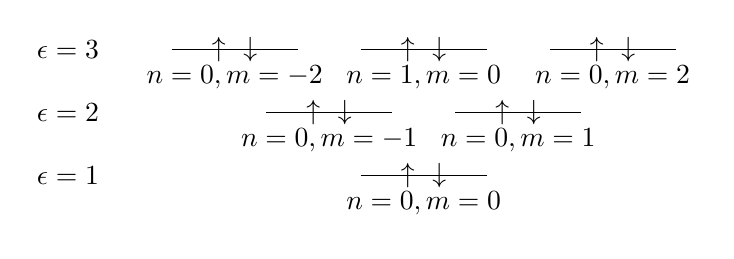
\begin{tikzpicture}[scale=0.8]
                        \begin{scope}
                            \foreach \i in {1, 2, 3} {
                                \draw(-1, \i - 1) node[anchor=east]
                                {$\epsilon = \i$};
                            }

                            % Highest energy level
                            \foreach \i in {0, 3, 6} {
                                \draw (\i, 2) -- (\i + 2, 2);
                                \node at (\i + 0.75, 2) {$\uparrow$};
                                \node at (\i + 1.25, 2) {$\downarrow$};
                            }
                            \node[below, inner sep=.2cm] at (1, 2)
                            {$n = 0, m = -2$};
                            \node[below, inner sep=.2cm] at (4, 2)
                            {$n = 1, m = 0$};
                            \node[below, inner sep=.2cm] at (7, 2)
                            {$n = 0, m = 2$};

                            % Middle energy level
                            \foreach \i in {1.5, 4.5} {
                                \draw (\i, 1) -- (\i + 2, 1);
                                \node at (\i + 0.75, 1) {$\uparrow$};
                                \node at (\i + 1.25, 1) {$\downarrow$};
                            }
                            \node[below, inner sep=.2cm] at (2.5, 1)
                            {$n = 0, m = -1$};
                            \node[below, inner sep=.2cm] at (5.5, 1)
                            {$n = 0, m = 1$};

                            % Lowest energy level
                            \draw (3, 0) -- (5, 0);
                            \node at (3 + 0.75, 0) {$\uparrow$};
                            \node at (3 + 1.25, 0) {$\downarrow$};
                            \node[below, inner sep=.2cm] at (4, 0)
                            {$n = 0, m = 0$};
                        \end{scope}
                    \end{tikzpicture}
                \end{center}
                \caption{In this plot we can see the energy degeneracy of the
                lowest three energy levels in the two-dimensional quantum dot.
                Each arrow representes a spin up or a spin down state with the
                quantum numbers $n$ and $m$ as listed below.}
                \label{fig:basis_states}
            \end{figure}

            Starting from the bottom and working our way upwards from left to
            right we can label each line from $0$ to $n$ in increasing
            order. This enumeration will serve as our common quantum number
            $\alpha$\footnote{Note that we use greek letters $\alpha, \beta,
            \dots$ for the harmonic oscillator wavefunctions as opposed to latin
            letters for the general indices.}. We will only work with full
            \emph{shells}, i.e., we restrict our views to systems of $N$
            particles where $N$ will be a magic number which we get by counting
            all spin states for each energy level and the energy levels below.
            In \autoref{fig:basis_states} we can see the magic number $N \in [2,
            6, 12]$.

            The normalization condition now reads
            \begin{align}
                \braket{\alpha}{\beta}
                = \delta_{\alpha\beta}\delta_{\sigma_\alpha\sigma_\beta},
            \end{align}
            The one-body matrix will be a diagonal matrix with the eigenenergies
            of the single particle harmonic oscillator functions as elements.
            \begin{align}
                \bra{\alpha}h\ket{\beta}
                = \epsilon_{\beta}
                \delta_{\alpha\beta}\delta_{\sigma_\alpha\sigma_\beta}.
            \end{align}

            The two-body matrix elements are a little harder to work out as the
            harmonic oscillator wavefunctions are not eigenfunctions to the
            correlation operator. Luckily, from E. Anisimovas and A.  Matulis
            (Equation A2)\cite{anisimovas1998energy} we can get an analytical
            expression for the two-body matrix elements. We can then construct
            the antisymmetric two-body matrix elements in the harmonic
            oscillator basis.
            \begin{align}
                \bra{\alpha\beta}\ket{\gamma\delta}
                &= \braket{\alpha\beta}{\gamma\delta}
                - \braket{\alpha\beta}{\delta\gamma}.
            \end{align}
            As we only need to compute these once it is a good idea to save all
            non-zero values of $\bra{\alpha\beta}\ket{\gamma\delta}$ to a file.

        \subsubsection{Constructing the Hartree-Fock basis}
            Having found the matrix elements of $h$ and $u$ we can now use the
            \emph{self-consistent field iteration} method to construct $h$ and
            $u$ in a \emph{restricted Hartree-Fock} basis. This will yield a
            better estimate to the actual, unknown basis functions of the
            system.

            % See Step 3 in:
            % http://sirius.chem.vt.edu/wiki/doku.php?id=crawdad:programming:project4

            The neatest, yet arguably the most abstract, way to write the Hartree-Fock
            equations for electron $i$\footnote{This is weird, as electron
            should be indistinguishable and therefor impossible to label.} is
            \begin{equation}
                f_i \varphi_i = \varepsilon_i \varphi_i,
            \end{equation}
            where $f_i$ is the Fock operator, $\varphi_i$ are eigenstates of the Fock
            operator consiting of a set of one-electorn wave funcitons, called the
            Hartree-Fock molecular orbitals, and $\varepsilon_i$ are the eigenenergies
            of the Fock operator. The fock operator, in matrix notation, is given by
            \begin{equation}
                F_{pa} = H_{pq} +  J(D)_{pq} - \frac{1}{2}K(D)_{pq},
            \end{equation}
            where $h_i$ is the one-body operatore, while the two-body operator is
            divided into what we call a direct part,
            \begin{equation}
                J(D)_{pq} = \braket{pq}{rs}D_{sr},
            \end{equation}
            and an exchange part,
            \begin{equation}
                K(D)_{pq} = \braket{ps}{rq}D_{sr}.
            \end{equation}
            The direct part of the two-body operator is comparable to classical Coloumb
            repulsion, while the exchange does not have a classical analog as it arises
            from the antisymmetry requirement of the wavefunction. $D_{sr}$ is the
            density matrix of the system.

            Introducing a basis set transforms the Hartree-Fock equations into the Rothaan
            equations
            \begin{equation}
                FC = SC\varepsilon.
            \end{equation}
            This is a generalised eigenvalue problem where $S$ serves as an overlap matrix
            that must be there in case of non-orthogonal basis. Since the Fock matrix $F$
            depends on it's own solution through the orbitals, the eigenvalue problem must
            be solved iteratively\footnote{This is also the reason why the
            Hartree-Fock-Roothaan equations are often called the self-consistent-field
            procedure.}

\section{Implementation}
    We have costructed a flexible framework for making performing Hartree-Fock 
    self-consistednt field (SCF) and coupled cluster with double excitations (CCD)
    computations. The entire code base consists of package for \lstinline{python}
    that is easy to install globally on any computer.
    
    Because we have employed a mixture of Python and C++ with Cython interfaces,
    the code sturcture may be difficult to undertand for someone without Cython
    experience, but we have neverteless tried to make the usage of the software as
    painless as possible.
    
    \subsection{Installation and Usage}

        The software is easy to install by first cloning the GitHub reopsitory,
        \begin{bash}
            git clone git@github.com:Schoyen/FYS4411.git
        \end{bash}
        Then all you need to do is change directory to the project code folder
        where a \lstinline{MakeFile} is included so you only need to build and
        install,
        \begin{bash}
            cd FYS4411/project_2/coupled-cluster
            make build
            make install
        \end{bash}
        Now everything should be able to run from anywhere on your computer.
        To ensure that all requirements of the program are satified you can
        install with \lstinline{make installr} instead.

        We have included a sample python script in \autoref{app:sample_script}
        that uses almost all methods and classes in the package. 

    \subsection{Program Structure}
        There are three main subsetions within our program structure,
        given in the directory tree below.

        \vspace{10pt}
        \dirtree{%
        .1 coupled\_cluster.
            .2 matrix\_elements.
                .3 generate\_matrices.
                .3 index\_map.
            .2 hartree\_fock.
                .3 scf\_rhf.
                .3 basis\_transformation.
            .2 schemes.
                .3 ccd.
                .3 ccd\_sparse.
                .3 ccd\_optimized.
        }
        \vspace{10pt}

        The first subsection, \mintinline{python}{matrix_elemtents},
        contains methods for computing matrix elements in harmonic
        oscillator basis from an analytical
        expression\cite{anisimovas1998energy}.  Computing the matrix
        elements is a very intensive task, and the central functions are
        therefore implemented in C++ with a Cython interface to enable use
        in Python.

        The \mintinline{python}{hartree_fock} subsection contains methods
        for changing from harmonic oscillator basis to Hartree-Fock basis as
        well as an implementation of the self-consistent-field algorithm to
        make this transaction possible.

        The \mintinline{python}{schemes} subsection is arguably the most
        important part of this project. The subsection has three different
        classes that perform the exact same computations, but in different
        and increasingly intelligent ways. First,
        \mintinline{python}{CoupledClusterDoubles} is the most
        straightforward and naïve way to solve the CCD amplitude equations.
        Second, because an overbearing amount of the elements in the
        operator matrices in this problem are zero, we have implemented a
        sparse matrix CDD solver in
        \mintinline{python}{CoupledClusterDoublesSparse}. Third,
        \mintinline{python}{CoupledClusterDoublesOptimized} takes advantage
        of sparse matrices as well, but is also parallellized and optimized
        with memory use and number of floating point operations in mind.

        Both in \mintinline{python}{CoupledClusterDoublesSparse} and
        \mintinline{python}{CoupledClusterDoublesOptimized} we make use
        of the intermediates in equations \ref{eq:intermediate1} to
        \ref{eq:intermediate4}. In the optimized class, special care was
        taken to compute

    \subsection{Convergence Problems and Mixing}

        Iterative many-body methods are prone to convergence problems for some
        configurations. Since Hartree-Fock is a variational method, SCF convergence
        is found when the energy is stationary with respect to inifitesimal 
        variations in the orbitals. Unfortunately, the SCF iteration scheme does 
        not always converge. Luckily, numerous techniques exist for controlling
        and accelerating convergence\cite{schlegel1991you}. The same kind of 
        methods have proven useful to ensure convergence of coupled cluster methods
        \cite{scuseria1986accelerating}.

        The simplest way to try to ``massage'' convergence out of the CCD-method 
        is to use \emph{damping} where you include a part of the result from the
        previous iteration i.e.,
        \begin{align}
            \tilde{t}^{k + 1} = \theta t^{k + 1} + (1 - \theta)t^k,
            \label{eq:mixing}
        \end{align}
        where $t^{k + 1}$ is the current value computed using
        \autoref{eq:iterative_amplitude} and $t^k$ is the previous value for the
        amplitude. Choosing $\theta \in [0, 1]$ we can tune how much of the
        previous amplitude we wish to include in the new state. This allows for
        a more gradual transition between the iterations. We now use
        $\tilde{t}^{k + 1}$ as our estimate of the new amplitude.

        A more sophisticated mixing method is the direct inversion 
        in the iterative subspace (DIIS), also known as Pulay mixing. While the
        common mixing method is used for many other applications
        \footnote{It is, for instance, called an alpha filter in data acquisition.},
        the DIIS method is developed with the sole intent of accelerating
        convergense in Hartree-Fock methods. In DIIS one would construct a
        linear combinations of approximate errors from previous iterations,
        analogous to a very clever weighted moving average. We have not implemented
        this scheme, but it nevertheless warrants mention.

\section{Results}

    \subsection{Ground state energies for two-dimensional quantum dots}
        Here we show the ground state energies for the two-dimensional quantum
        dots using restriced Hartree-Fock (RHF), coupled cluster doubles using
        both the harmonic oscillator basis and the Hartree-Fock basis which we
        construct after running the RHF-method. We have chosen the convergence
        criteria to be $\num{1e-6}$ in our results for the sake of comparison
        with M. P. Lohne\cite{lohne2011ab}.

        % TODO: Add short introduction to each table and link to them. Leave the
        % discussion of the results in the discussion section.

    \begin{table}
        \centering
        \caption{Results for N = 2 particles, where convergence was 
            acchieved for all parameters. Taut's\cite{taut1994two}
            analytic result for $\omega=1.0a.u.$ is $3$.}
        \begin{ruledtabular}
            \begin{tabular}{c|c|ccc}
                $\omega$ & $R$ & RHF & CCD(HO) & CCD(HF) \\
                \hline
                           &  $1$  & $0.596333$ & $0.596333$ & $0.596333$ \\
                           &  $2$  & $0.596333$ & $0.512520$ & $0.512520$ \\
                           &  $3$  & $0.526903$ & $0.505972$ & $0.442235$ \\
                           &  $4$  & $0.526903$ & $0.499216$ & $0.442011$ \\
                           &  $5$  & $0.525666$ & $0.497172$ & $0.443293$ \\
    \multirow{2}{*}{$0.1$} &  $6$  & $0.525666$ & $0.494232$ & $0.443145$ \\
                           &  $7$  & $0.525635$ & $0.493142$ & $0.443056$ \\
                           &  $8$  & $0.525635$ & $0.491895$ & $0.442981$ \\
                           &  $9$  & $0.525635$ & $0.491262$ & $0.442927$ \\
                           &  $10$ & $0.525635$ & $0.490649$ & $0.442886$ \\
                           &  $11$ & $0.525635$ & $0.490262$ & $0.442853$ \\
                           &  $12$ & $0.525635$ & $0.489918$ & $0.442827$ \\
                \hline

                           &  $1$  & $1.886227$ & $1.886227$ & $1.886227$ \\
                           &  $2$  & $1.886227$ & $1.786914$ & $1.786914$ \\
                           &  $3$  & $1.799856$ & $1.778903$ & $1.681979$ \\
                           &  $4$  & $1.799856$ & $1.760117$ & $1.673881$ \\
                           &  $5$  & $1.799748$ & $1.754385$ & $1.670053$ \\
    \multirow{2}{*}{$0.5$} &  $6$  & $1.799748$ & $1.748232$ & $1.667804$ \\
                           &  $7$  & $1.799745$ & $1.745231$ & $1.666474$ \\
                           &  $8$  & $1.799745$ & $1.742548$ & $1.665494$ \\
                           &  $9$  & $1.799743$ & $1.740860$ & $1.664805$ \\
                           &  $10$ & $1.799743$ & $1.739444$ & $1.664270$ \\
                           &  $11$ & $1.799742$ & $1.738416$ & $1.663856$ \\
                           &  $12$ & $1.799742$ & $1.737562$ & $1.663522$ \\
                \hline

                           &  $1$  & $3.253314$ & $3.253314$ & $3.253314$ \\
                           &  $2$  & $3.253314$ & $3.152328$ & $3.152328$ \\
                           &  $3$  & $3.162691$ & $3.141827$ & $3.039048$ \\
                           &  $4$  & $3.162691$ & $3.118679$ & $3.025273$ \\
                           &  $5$  & $3.161921$ & $3.110967$ & $3.017944$ \\
    \multirow{2}{*}{$1.0$} &  $6$  & $3.161921$ & $3.103338$ & $3.013923$ \\
                           &  $7$  & $3.161909$ & $3.099324$ & $3.011405$ \\
                           &  $8$  & $3.161909$ & $3.095916$ & $3.009621$ \\
                           &  $9$  & $3.161909$ & $3.093662$ & $3.008343$ \\
                           &  $10$ & $3.161909$ & $3.091818$ & $3.007357$ \\
                           &  $11$ & $3.161909$ & $3.090436$ & $3.006590$ \\
                           &  $12$ & $3.161909$ & $3.089299$ & $3.005970$ \\
                \hline

                           &  $1$  & $5.772454$ & $5.772454$ & $5.772454$ \\
                           &  $2$  & $5.772454$ & $5.671234$ & $5.671234$ \\
                           &  $3$  & $5.679048$ & $5.658272$ & $5.553528$ \\
                           &  $4$  & $5.679048$ & $5.631669$ & $5.534333$ \\
                           &  $5$  & $5.677282$ & $5.622092$ & $5.523490$ \\
    \multirow{2}{*}{$2.0$} &  $6$  & $5.677282$ & $5.613118$ & $5.517552$ \\
                           &  $7$  & $5.677206$ & $5.608130$ & $5.513709$ \\
                           &  $8$  & $5.677206$ & $5.604026$ & $5.511012$ \\
                           &  $9$  & $5.677204$ & $5.601216$ & $5.509050$ \\
                           &  $10$ & $5.677204$ & $5.598946$ & $5.507540$ \\
                           &  $11$ & $5.677204$ & $5.597213$ & $5.506356$ \\
                           &  $12$ & $5.677204$ & $5.595791$ & $5.505399$
            \end{tabular}
        \end{ruledtabular}
        \label{tab:N2}
    \end{table}

    \begin{table}
        \centering
        \caption{Results for $N = 6$ particles. No convergence for HO
            basis for low frequency and large number of shells.}
        \begin{ruledtabular}
            \begin{tabular}{c|c|ccc}
                $\omega$ & $R$ & RHF & CCD(HO) & CCD(HF) \\ \hline
                         &  $2$  & $4.864244$ & $4.864244$ & $4.864244$ \\
                         &  $3$  & $4.435740$ & $4.446235$ & $4.319901$ \\
                         &  $4$  & $4.019787$ & $4.383692$ & $3.829962$ \\
                         &  $5$  & $3.963149$ & \nan & $3.666722$ \\
                         &  $6$  & $3.870617$ & \nan & $3.597876$ \\
                  $0.1$  &  $7$  & $3.863135$ & \nan & $3.590388$ \\
                         &  $8$  & $3.852880$ & \nan & $3.587711$ \\
                         &  $9$  & $3.852591$ & \nan & $3.587291$ \\
                         &  $10$ & $3.852393$ & \nan & $3.587136$ \\
                         &  $11$ & $3.852391$ & \nan & $3.586821$ \\
                         &  $12$ & $3.852382$ & \nan & $3.586582$ \\ \hline

                         &  $2$  & $13.640713$ & $13.640713$ & $13.640713$ \\
                         &  $3$  & $13.051620$ & $13.385987$ & $12.901520$ \\
                         &  $4$  & $12.357471$ & $13.261097$ & $12.057345$ \\
                         &  $5$  & $12.325128$ & $13.138572$ & $11.934988$ \\
                         &  $6$  & $12.271499$ & $13.084158$ & $11.864098$ \\
                  $0.5$  &  $7$  & $12.271375$ & $13.068399$ & $11.849762$ \\
                         &  $8$  & $12.271361$ & $13.055561$ & $11.841330$ \\
                         &  $9$  & $12.271337$ & $13.045386$ & $11.835470$ \\
                         &  $10$ & $12.271326$ & $13.037878$ & $11.831351$ \\
                         &  $11$ & $12.271324$ & \nan & $11.828242$ \\
                         &  $12$ & $12.271320$ & \nan & $11.825835$ \\ \hline

                         &  $2$  & $22.219813$ & $22.219813$ & $22.219813$ \\
                         &  $3$  & $21.593198$ & $21.974675$ & $21.423811$ \\
                         &  $4$  & $20.766919$ & $21.854191$ & $20.429265$ \\
                         &  $5$  & $20.748402$ & $21.793624$ & $20.332454$ \\
                         &  $6$  & $20.720257$ & $21.750091$ & $20.274013$ \\
                  $1.0$  &  $7$  & $20.720132$ & $21.718843$ & $20.249849$ \\
                         &  $8$  & $20.719248$ & $21.695224$ & $20.234705$ \\
                         &  $9$  & $20.719248$ & $21.675931$ & $20.224389$ \\
                         &  $10$ & $20.719217$ & $21.661830$ & $20.217075$ \\
                         &  $11$ & $20.719215$ & $21.649812$ & $20.211541$ \\
                         &  $12$ & $20.719215$ & $21.640765$ & $20.207258$ \\
                         \hline

                         &  $2$  & $37.281425$ & $37.281425$ & $37.281425$ \\
                         &  $3$  & $36.637217$ & $37.042127$ & $36.450634$ \\
                         &  $4$  & $35.689555$ & $36.925664$ & $35.328432$ \\
                         &  $5$  & $35.681729$ & $36.864367$ & $35.250185$ \\
                         &  $6$  & $35.672333$ & $36.812895$ & $35.200308$ \\
                  $2.0$  &  $7$  & $35.671851$ & $36.775986$ & $35.168245$ \\
                         &  $8$  & $35.670358$ & $36.747864$ & $35.147097$ \\
                         &  $9$  & $35.670333$ & $36.725261$ & $35.131953$ \\
                         &  $10$ & $35.670144$ & $36.708362$ & $35.121033$ \\
                         &  $11$ & $35.670143$ & $36.694188$ & $35.112680$ \\
                         &  $12$ & $35.670127$ & $36.683281$ & $35.106188$
            \end{tabular}
        \end{ruledtabular}
        \label{tab:N6}
    \end{table}

    \begin{table}
        \centering
        \caption{Here we look at $N = 12$ particles ($R = 3$ shells).  We did
        not achieve convergence using the harmonic oscillator basis for the
        lower frequency values and large number of shells.}
        \begin{ruledtabular}
            \begin{tabular}{c|c|ccc}
                $\omega$ & $R$ & RHF & CCD(HO) & CCD(HF) \\
                \hline
                      & $3$ & $46.361130$ & $46.361130$ & $46.361130$ \\
                      & $4$ & $43.663267$ & $45.837079$ & $43.309845$ \\
                      & $5$ & $41.108851$ & $45.456883$ & $40.654710$ \\
                      & $6$ & $40.750512$ & \nan & $40.068340$ \\
                $0.5$ & $7$ & $40.302719$ & \nan & $39.508500$ \\
                      & $8$ & $40.263752$ & \nan & $39.399128$ \\
                      & $9$ & $40.216688$ & \nan & $39.329311$ \\
                      & $10$ & $40.216252$ & \nan & $39.309409$ \\
                      & $11$ & $40.216195$ & \nan & $39.296007$ \\
                      & $12$ & $40.216165$ & \nan & $39.285968$ \\
                \hline
                      & $3$ & $73.765549$ & $73.765549$ & $73.765549$ \\
                      & $4$ & $70.673849$ & $73.314476$ & $70.324250$ \\
                      & $5$ & $67.569930$ & $72.990679$ & $67.031096$ \\
                      & $6$ & $67.296869$ & \nan & $66.526677$ \\
                $1.0$ & $7$ & $66.934745$ & \nan & $66.049564$ \\
                      & $8$ & $66.923094$ & \nan & $65.972157$ \\
                      & $9$ & $66.912244$ & \nan & $65.921205$ \\
                      & $10$ & $66.912035$ & \nan & $65.889281$ \\
                      & $11$ & $66.911365$ & \nan & $65.866715$ \\
                      & $12$ & $66.911364$ & \nan & $65.849776$ \\
                \hline
                      & $3$ & $120.722260$ & $120.722260$ & $120.722260$ \\
                      & $4$ & $117.339642$ & $120.296556$ & $116.995036$ \\
                      & $5$ & $113.660396$ & $120.007146$ & $113.048934$ \\
                      & $6$ & $113.484866$ & $119.759037$ & $112.658821$ \\
                $2.0$ & $7$ & $113.247601$ & $119.662199$ & $112.309482$ \\
                      & $8$ & $113.246579$ & $119.584733$ & $112.235521$ \\
                      & $9$ & $113.246303$ & $119.524394$ & $112.181828$ \\
                      & $10$ & $113.245854$ & $119.472283$ & $112.140661$ \\
                      & $11$ & $113.245256$ & $119.430353$ & $112.109973$ \\
                      & $12$ & $113.245183$ & $119.394712$ & $112.085683$ \\
                \hline
                $5.0$ & $3$ & $242.334879$ & $242.334879$ & $242.334879$ \\
                      & $4$ & $238.739591$ & $241.927593$ & $238.394598$ \\
                      & $5$ & $234.352741$ & $241.663950$ & $233.680649$ \\
                      & $6$ & $234.282331$ & $241.507595$ & $233.425243$ \\
                      & $7$ & $234.194820$ & $241.390525$ & $233.226529$ \\
                      & $8$ & $234.194059$ & $241.293417$ & $233.137933$ \\
                      & $9$ & $234.190797$ & $241.221056$ & $233.070205$ \\
                      & $10$ & $234.190714$ & $241.158896$ & $233.020009$ \\
                      & $11$ & $234.190665$ & $241.109926$ & $232.980634$ \\
                      & $12$ & $234.190553$ & $241.068091$ & $232.948528$
            \end{tabular}
        \end{ruledtabular}
        \label{tab:N12}
    \end{table}

    \begin{table}
        \centering
        \caption{In this table we look at $N = 20$ particles ($R = 4$ shells).
        We did not achieve convergence using the harmonic oscillator basis for
        the lower frequency values and large number of shells.}
        \begin{ruledtabular}
            \begin{tabular}{c|c|ccc}
                $\omega$ & $R$ & RHF & CCD(HO) & CCD(HF) \\
                \hline
                $1.0$ & $4$ & $177.963297$ & $177.963297$ & $177.963297$ \\
                      & $5$ & $168.792442$ & $177.206536$ & $168.459124$ \\
                      & $6$ & $161.339721$ & \nan & $160.594507$ \\
                      & $7$ & $159.958722$ & \nan & $158.841120$ \\
                      & $8$ & $158.400172$ & \nan & $157.038330$ \\
                      & $9$ & $158.226030$ & \nan & $156.676039$ \\
                      & $10$ & $158.017667$ & \nan & $156.367930$ \\
                      & $11$ & $158.010276$ & \nan & $156.292422$ \\
                      & $12$ & $158.004951$ & \nan & $156.238258$ \\
                \hline
                $2.0$ & $4$ & $286.825295$ & $286.825295$ & $286.825295$ \\
                      & $5$ & $276.898196$ & $286.159148$ & $276.381708$ \\
                      & $6$ & $267.269712$ & $285.614958$ & $266.413122$ \\
                      & $7$ & $266.213200$ & \nan & $264.969415$ \\
                      & $8$ & $264.933622$ & \nan & $263.434546$ \\
                      & $9$ & $264.874009$ & \nan & $263.215451$ \\
                      & $10$ & $264.809954$ & \nan & $263.046195$ \\
                      & $11$ & $264.809901$ & \nan & $262.963703$ \\
                      & $12$ & $264.809306$ & \nan & $262.899698$ \\
                \hline
                $5.0$ & $4$ & $563.773952$ & $563.773952$ & $563.773952$ \\
                      & $5$ & $552.630093$ & $563.160136$ & $552.118708$ \\
                      & $6$ & $540.804720$ & $562.692231$ & $539.824400$ \\
                      & $7$ & $540.227793$ & $562.306123$ & $538.886074$ \\
                      & $8$ & $539.499326$ & $562.114279$ & $537.925127$ \\
                      & $9$ & $539.495941$ & \nan & $537.769045$ \\
                      & $10$ & $539.494611$ & \nan & $537.646668$ \\
                      & $11$ & $539.493513$ & \nan & $537.548828$ \\
                      & $12$ & $539.491764$ & \nan & $537.470616$ \\
                \hline
                $10.0$ & $4$ & $973.032700$ & $973.032700$ & $973.032700$ \\
                       & $5$ & $961.371081$ & $972.439478$ & $960.862053$ \\
                       & $6$ & $948.057077$ & $972.002302$ & $947.019789$ \\
                       & $7$ & $947.765474$ & $971.716015$ & $946.399546$ \\
                       & $8$ & $947.410305$ & $971.508584$ & $945.827806$ \\
                       & $9$ & $947.409440$ & $971.332133$ & $945.663820$ \\
                       & $10$ & $947.404930$ & $971.193592$ & $945.528489$ \\
                       & $11$ & $947.404361$ & $971.076617$ & $945.424175$ \\
                       & $12$ & $947.403875$ & $970.978571$ & $945.339080$ \\
            \end{tabular}
        \end{ruledtabular}
        \label{tab:N20}
    \end{table}

\section{Discussion}

    \subsection{Validity of results}
        The analytical computed energy for $\omega=1.0a.u.$
        and $N=2$ is $3$\cite{taut1994two}. From our tables we see 
        that RHF is least successful in reaching this value, CCD in
        HF basis is best, while CCD with HO basis is generally somewhere 
        between the two. We see that we get even closer to the analytical
        ``truth'' by increasing the number of shells.

        The rest of results have been compared with the master thesis of M. P.
        Lohne\cite{lohne2010coupled} for up to 10 shells. Lohne gets two sets of
        energies, one set from RHF and one set from CCSD code with harmonic
        oscillator basis functions. Our CCD code with Hartree-Fock basis will
        for some configurations\footnote{By configurations we mean frequency
        $\omega$ and number of particles $N$.} beat CCSD with plain harmonic
        oscillator basis. For 12 shells we can compare with the results from M.
        P. Lohne et al.\cite{lohne2011ab}, but in this article an
        \emph{effective interaction} for the Hamiltonian with a CCSD code has
        been used. These results are therefore significanlty better than ours,
        but we can get a ``ball-park'' idea to benchmark against.

    \subsection{Convergence trouble}
        For a large number of particles and a low frequency the CCD-method get
        trouble with convergence. This happens as the confining potential $v
        \propto \omega^2$ will not be able to confine the particles when the
        interaction gets too strong. The CCD-method will in particular get a
        hard time keep the particles together as the excitation operator $t$
        only excites pairs of particles leading to a too strong increase in the
        interaction when the particles increase their energy level. This effect
        can potentially be somewhat alleviated by including the singles
        excitation, e.g., using the CCSD-method.

        We can see this behaviour in our results. For $N = 2$ we get convergence
        for all methods for $\omega = 0.1$ shown in \autoref{tab:N2}. By
        increasing to $N = 6$ particles we immediately see how CCD with the HO
        basis will get in trouble for small values of $\omega$. Even by increasing
        the strength of the confinment this method does converge.

        For $N = 6$ none of the methods converged when $\omega =
        0.1$\footnote{The RHF-method would probably have converged if we had
        started tuning its mixing parameter, but as we have focused on CCD we did
        not think it relevant to include these results.}. By increasing the
        frequency we restored the convergence. For larger number of shells we
        had to start increasing the value of $\theta \to 0.9$ in order to get
        convergence within the threshold.

        CCD with HO basis experiences the same convergence problems also for,
        $N=12$ particles and for $N=20$ particles.

    \subsection{Sparse implementation}

\appendix
\section{The normal ordered Hamiltonian}
    When constructing the normal ordered Hamiltonian we use Wick's theorem to
    write the one-body, $h$, and the two-body, $u$, operators onto a normal
    ordered form. Specifically we define the normal ordered form in terms of the
    \emph{Fermi vacuum}\footnote{Fermi vacuum defines the reference state, i.e.,
    $\kslat$, as the vacuum.}. That is, an operator on normal ordered form
    destroys the reference Slater determinant.

    We start by writing the one-body operator, $h$, to its normal-ordered form.
    \begin{align}
        h &= \sum_{pq}h^p_q\acr{p}\ade{q}
        = \sum_{pq}h^p_q\para{
            \{\acr{p}\ade{q}\}
            + \{
                \wick{\c a_{p}^{\dagger} \c a_{q}}
            \}
        }
        \\
        &= \sum_{pq}h^p_q\{
            \acr{p}\ade{q}
        \}
        + \sum_{pq}h^p_q\delta_{p \in i}\delta_{pq}
        \\
        &= h_N + \sum_{i}h^i_i,
    \end{align}
    where we have used $\delta_{p \in i}$ to mean that $p$ must be an occupied
    index. Doing the same for the two-body operator is a slightly more tedious
    endeavor. For brevity we will only write out the operator strings and only
    keep the non-zero contributions.
    \begin{align}
        \acr{p}\acr{q}\ade{s}\ade{r}
        &=
        \{\acr{p}\acr{q}\ade{s}\ade{r}\}
        + \{
            \wick{\c a_p^{\dagger} a_{q}^{\dagger} \c a_{s} a_{r}}
        \}
        + \{
            \wick{\c a_p^{\dagger} a_{q}^{\dagger} a_{s} \c a_{r}}
        \}
        \nonumber \\
        &\qquad
        + \{
            \wick{a_p^{\dagger} \c a_{q}^{\dagger} \c a_{s} a_{r}}
        \}
        + \{
            \wick{a_p^{\dagger} \c a_{q}^{\dagger} a_{s} \c a_{r}}
        \}
        \nonumber \\
        &\qquad
        + \{
            \wick{\c1 a_p^{\dagger} \c2 a_{q}^{\dagger} \c1 a_{s} \c2 a_{r}}
        \}
        + \{
            \wick{\c2 a_p^{\dagger} \c1 a_{q}^{\dagger} \c1 a_{s} \c2 a_{r}}
        \}
        \\
        &=
        \{\acr{p}\acr{q}\ade{s}\ade{r}\}
        - \delta_{p \in i}\delta_{ps}\{\acr{q}\ade{r}\}
        + \delta_{p \in i}\delta_{pr}\{\acr{q}\ade{s}\}
        \nonumber \\
        &\qquad
        + \delta_{q \in i}\delta_{qs}\{\acr{p}\ade{r}\}
        - \delta_{q \in i}\delta_{qr}\{\acr{p}\ade{s}\}
        \nonumber \\
        &\qquad
        - \delta_{p \in i}\delta_{ps}\delta_{q \in j}\delta_{qr}
        + \delta_{p \in i}\delta_{pr}\delta_{q \in j}\delta_{qs}.
    \end{align}
    Inserted into the full two-body operator and sorting out the sums we get
    \begin{align}
        u
        &=
        \frac{1}{4}\sum_{pqrs}\bra{pq}\ket{rs}
        \{\acr{p}\acr{q}\ade{s}\ade{r}\}
        - \frac{1}{4}\sum_{iqr}\bra{iq}\ket{ri}\{\acr{q}\ade{r}\}
        \nonumber \\
        &\qquad
        + \frac{1}{4}\sum_{iqs}\bra{iq}\ket{is}\{\acr{q}\ade{s}\}
        + \frac{1}{4}\sum_{pir}\bra{pi}\ket{ri}\{\acr{p}\ade{r}\}
        \nonumber \\
        &\qquad
        - \frac{1}{4}\sum_{pis}\bra{pi}\ket{is}\{\acr{p}\ade{s}\}
        - \frac{1}{4}\sum_{ij}\bra{ij}\ket{ji}
        \nonumber \\
        &\qquad
        + \frac{1}{4}\sum_{ij}\bra{ij}\ket{ij}.
    \end{align}
    Using the antisymmetric properties of the two-body matrix elements,
    \begin{align}
        \bra{pq}\ket{rs}
        = - \bra{pq}\ket{sr}
        = - \bra{qp}\ket{rs}
        = \bra{qp}\ket{sr},
    \end{align}
    and relabeling of the indices we can rearrange and collect some terms.
    \begin{align}
        u
        &=
        W_N + \sum_{pir}\bra{pi}\ket{ri}\{\acr{p}\ade{r}\}
        + \half\sum_{ij}\bra{ij}\ket{ij},
    \end{align}
    where the normal ordered two-body operator is
    \begin{align}
        W_N = \frac{1}{4}\sum_{pqrs}
        \bra{pq}\ket{rs}\{\acr{p}\acr{q}\ade{s}\ade{r}\}.
    \end{align}
    When we now construct the full Hamiltonian we can collect some terms. The
    constants in both the one-body and the two-body operator in total constitues
    the reference energy.
    \begin{align}
        E_0 \equiv \bslat H\kslat
        = \sum_{i}h_i^i + \frac{1}{2}\sum_{ij}\bra{ij}\ket{ij}.
        \label{eq:reference_energy}
    \end{align}
    Combining the normal ordered one-body operator and the second term in the
    two-body operator, i.e., the term with a single creation and annihilation
    operator pair, we get the normal ordered Fock-operator.
    \begin{align}
        F_N
        &=
        \sum_{pq}h_{q}^{p}\{\acr{p}\ade{q}\}
        + \sum_{pqi}\bra{pi}\ket{qi}\{\acr{p}\ade{q}\}
        \\
        &= \sum_{pq}f_{q}^{p}\{\acr{p}\ade{q}\},
    \end{align}
    where we have defined the Fock matrix elements as
    \begin{align}
        f_{q}^{p}
        &=
        h_q^p + \sum_{i}\bra{pi}\ket{qi}.
    \end{align}
    In total we get the full Hamiltonian
    \begin{align}
        H
        &=
        F_N + W_N + \bslat H\kslat
        \\
        &= H_N + \bslat H\kslat,
    \end{align}
    which is what we wanted to show.\cite{crawford2007introduction}

\section{Amplitude Equations}

    \label{app:wickOnAmplitude}

    In this section we have provided a few sample computations of how one would
    evaluate the amplitude equations using wicks theorem. Starting with the simplest
    term including only the normal-ordered Hamiltonian,

    \begin{equation}
        \begin{aligned}
            \bra{\Phi_{ij}^{ab}} &(F_N + V_N)\ket{\Phi_0} \\
             =& \sum_{pq}f_{pq}\bra{\Phi_0}\{a_i^\dagger a_j^\dagger a_ba_a\}\{a^\dagger_pa_q\}\ket{\Phi_0} \\
             &+\frac{1}{4}\sum_{pqrs}\bra{pq}\ket{rs}
             \bra{\Phi_0}\{a_i^\dagger a_j^\dagger a_ba_a\}\{a^\dagger_pa^\dagger_qa_sa_r\}\ket{\Phi_0}.
        \end{aligned}
        \end{equation}
        The one-electron component does not have any full contractions, while the
        two-electron component produces one contributing integral,
        \begin{equation}
        \begin{aligned}
            \bra{\Phi_{ij}^{ab}} &(V_N)\ket{\Phi_0} \\
                =& \frac{1}{4}\sum_{pqrs}\bra{pq}\ket{rs}
             \bra{\Phi_0}\{a_i^\dagger a_j^\dagger a_ba_a\}\{a^\dagger_pa^\dagger_qa_sa_r\}\ket{\Phi_0} \\
                 =& \frac{1}{4} \sum_{pqrs} \bra{pq}\ket{rs} \\ &\times\Big(
                     \{ \wick{\c1 a^\dagger_i \c2 a^\dagger_j \c3 a_b \c4 a_a
                     \c4 a^\dagger_p \c3 a^\dagger_q \c2 a_s \c1 a_r}\}
                     +
                     \{ \wick{\c1 a^\dagger_i \c2 a^\dagger_j \c4 a_b \c3 a_a
                     \c4 a^\dagger_p \c3 a^\dagger_q \c2 a_s \c1 a_r}\} \\
                   &\ +
                      \{ \wick{\c2 a^\dagger_i \c1 a^\dagger_j \c3 a_b \c4 a_a
                     \c4 a^\dagger_p \c3 a^\dagger_q \c2 a_s \c1 a_r}\}
                     +
                     \{ \wick{\c2 a^\dagger_i \c1 a^\dagger_j \c4 a_b \c3 a_a
                     \c4 a^\dagger_p \c3 a^\dagger_q \c2 a_s \c1 a_r}\}
                 \Big) \\
                 =&  \frac{1}{4} \sum_{pqrs} \bra{pq}\ket{rs}
                 ( \delta_{ap}\delta_{bq}\delta_{js}\delta_{ir}
                  -\delta_{aq}\delta_{bp}\delta_{js}\delta_{ir} \\
                 &\ -\delta_{ap}\delta_{bq}\delta_{jr}\delta_{is}
                  +\delta_{aq}\delta_{bp}\delta_{jr}\delta_{is}) \\
                  =& \bra{ab}\ket{ij} = u^{ab}_{ij}.
        \end{aligned}
        \end{equation}

        Next we would like to evaluate $\bra{\Phi_{ij}^{ab}}(F_N + V_N)T_2\ket{\Phi_0}$. Starting with the
        term involving the Fock operator $F_N$,
        \begin{equation}
        \begin{aligned}
            \bra{\Phi_{ij}^{ab}}&F_NT_2\ket{\Phi_0} \\
                =& \frac{1}{4}\sum_{pq}\sum_{klcd}f_{pq}t_{kl}^{cd} \bra{\Phi_0}
                    \{a_i^\dagger a_j^\dagger a_b a_a \}(\{a^\dagger_pa_q \}\{a^\dagger_c a^\dagger_d a_l a_k \})_c \ket{\Phi_0} \\
                =& \frac{1}{4}\sum_{pq}\sum_{klcd}f_{pq} t_{kl}^{cd} \\
                \times \Big(
                    &\{\wick{\c1 a^\dagger_i \c2 a^\dagger_j \c3 a_b \c4 a_a \c5 a^\dagger_p \c2 a_q \c3 a^\dagger_c \c4 a^\dagger_d \c1 a_l \c5 a_k } \}
                 + \{\wick{\c1 a^\dagger_i \c2 a^\dagger_j \c3 a_b \c4 a_a \c5 a^\dagger_p \c1 a_q \c3 a^\dagger_c \c4 a^\dagger_d \c2 a_l \c5 a_k } \}    \\
                + &\{\wick{\c1 a^\dagger_i \c2 a^\dagger_j \c3 a_b \c4 a_a \c5 a^\dagger_p \c2 a_q \c4 a^\dagger_c \c3 a^\dagger_d \c1 a_l \c5 a_k } \}
                 + \{\wick{\c1 a^\dagger_i \c2 a^\dagger_j \c3 a_b \c4 a_a \c5 a^\dagger_p \c1 a_q \c4 a^\dagger_c \c3 a^\dagger_d \c2 a_l \c5 a_k } \} \\
                + &\{\wick{\c1 a^\dagger_i \c2 a^\dagger_j \c3 a_b \c4 a_a \c5 a^\dagger_p \c1 a_q \c3 a^\dagger_c \c4 a^\dagger_d \c5 a_l \c2 a_k } \}
                  + \{\wick{\c1 a^\dagger_i \c2 a^\dagger_j \c3 a_b \c4 a_a \c5 a^\dagger_p \c1 a_q \c4 a^\dagger_c \c3 a^\dagger_d \c5 a_l \c2 a_k } \} \\
                + &\{\wick{\c1 a^\dagger_i \c2 a^\dagger_j \c3 a_b \c4 a_a \c5 a^\dagger_p \c2 a_q \c3 a^\dagger_c \c4 a^\dagger_d \c5 a_l \c1 a_k } \}
                  + \{\wick{\c1 a^\dagger_i \c2 a^\dagger_j \c3 a_b \c4 a_a \c5 a^\dagger_p \c2 a_q \c4 a^\dagger_c \c3 a^\dagger_d \c5 a_l \c1 a_k } \} \\
                + &\{\wick{\c1 a^\dagger_i \c2 a^\dagger_j \c3 a_b \c4 a_a \c3 a^\dagger_p \c5 a_q \c5 a^\dagger_c \c4 a^\dagger_d \c2 a_l \c1 a_k } \}
                  + \{\wick{\c1 a^\dagger_i \c2 a^\dagger_j \c3 a_b \c4 a_a \c3 a^\dagger_p \c5 a_q \c5 a^\dagger_c \c4 a^\dagger_d \c1 a_l \c2 a_k } \} \\
                + &\{\wick{\c1 a^\dagger_i \c2 a^\dagger_j \c3 a_b \c4 a_a \c4 a^\dagger_p \c5 a_q \c5 a^\dagger_c \c3 a^\dagger_d \c2 a_l \c1 a_k } \}
                  +\{\wick{\c1 a^\dagger_i \c2 a^\dagger_j \c3 a_b \c4 a_a \c4 a^\dagger_p \c5 a_q \c5 a^\dagger_c \c3 a^\dagger_d \c1 a_l \c2 a_k } \} \\
                + &\{\wick{\c1 a^\dagger_i \c2 a^\dagger_j \c3 a_b \c4 a_a \c3 a^\dagger_p \c5 a_q \c4 a^\dagger_c \c5 a^\dagger_d \c1 a_l \c2 a_k } \}
                  +\{\wick{\c1 a^\dagger_i \c2 a^\dagger_j \c3 a_b \c4 a_a \c3 a^\dagger_p \c5 a_q \c4 a^\dagger_c \c5 a^\dagger_d \c2 a_l \c1 a_k } \} \\
                + &\{\wick{\c1 a^\dagger_i \c2 a^\dagger_j \c3 a_b \c4 a_a \c3 a^\dagger_p \c5 a_q \c4 a^\dagger_c \c5 a^\dagger_d \c1 a_l \c2 a_k } \}
                  + \{\wick{\c1 a^\dagger_i \c2 a^\dagger_j \c3 a_b \c4 a_a \c4 a^\dagger_p \c5 a_q \c3 a^\dagger_c \c5 a^\dagger_d \c2 a_l \c1 a_k } \}
                \Big) \\
                =& \sum_{pq}\sum_{klcd}f_{pq} t_{kl}^{cd} \\
                \times&( - \delta_{a c} \delta_{b d} \delta_{i k} \delta_{j q} \delta_{l p} + \delta_{a c} \delta_{b d} \delta_{i l} \delta_{j q} \delta_{k p}  \\
                 \ &+ \delta_{a c} \delta_{b d} \delta_{i q} \delta_{j k} \delta_{l p} - \delta_{a c} \delta_{b d} \delta_{i q} \delta_{j l} \delta_{k p} \\
                 \ &+ \delta_{a c} \delta_{b p} \delta_{d q} \delta_{i k} \delta_{j l} - \delta_{a c} \delta_{b p} \delta_{d q} \delta_{i l} \delta_{j k} \\
                 \ & + \delta_{a d} \delta_{b c} \delta_{i k} \delta_{j q} \delta_{l p} - \delta_{a d} \delta_{b c} \delta_{i l} \delta_{j q} \delta_{k p} \\
                 \ &- \delta_{a d} \delta_{b c} \delta_{i q} \delta_{j k} \delta_{l p} + \delta_{a d} \delta_{b c} \delta_{i q} \delta_{j l} \delta_{k p} \\
                 \ &- \delta_{a d} \delta_{b p} \delta_{c q} \delta_{i k} \delta_{j l} + \delta_{a d} \delta_{b p} \delta_{c q} \delta_{i l} \delta_{j k} \\
                 \ &- \delta_{a p} \delta_{b c} \delta_{d q} \delta_{i k} \delta_{j l} + \delta_{a p} \delta_{b c} \delta_{d q} \delta_{i l} \delta_{j k} \\
                 \ &+ \delta_{a p} \delta_{b d} \delta_{c q} \delta_{i k} \delta_{j l} - \delta_{a p} \delta_{b d} \delta_{c q} \delta_{i l} \delta_{j k}) \\
                 =& (f_{bc}t^{ac}_{ij} - f_{ac}t^{bc}_{ij}) - (f_{jk}t^{ab}_{ik} - f_{ik}t^{ab}_{jk}) \\
                 =& f_{bc}t^{ac}_{ij}P(ab) - f_{kj}t^{ab}_{ik}P(ij)
        \end{aligned}
        \end{equation}
        Where in the last steps we have consigned the sums by Einstein summation notation.
\section{Finding Amplitude Equation Intermediates}
    Starting from the CCD amplitude equation we factor out terms that will have the same
    indices if we contract them,
    \begin{align}
        &\begin{aligned}
        0 =& u^{ab}_{ij} + f^b_c t^{ac}_{ij}P(ab) - f^k_jt^{ab}_{ik}P(ij) \\
          &+ \frac{1}{4}t^{cd}_{ij} t^{ab}_{mn} u^{mn}_{cd} + \frac{1}{2}t^{cd}_{ij} u^{ab}_{cd} \\
          &+ \frac{1}{2}t^{cd}_{jm} t^{ab}_{in} u^{mn}_{cd} P(ij) - \frac{1}{2}t^{ac}_{nm} t^{bd}_{ij} u^{nm}_{cd} P(ab) \\
          &+ t^{ac}_{im} t^{bd}_{jn} u^{mn}_{cd} P(ij) + t^{ac}_{im} u^{bm}_{jc} P(ab) P(ij) \\
          &+ \frac{1}{2}t^{ab}_{im} u^{mn}_{jn},
        \end{aligned}\\
        &\begin{aligned}
        0 =& u^{ab}_{ij} + f^b_c t^{ac}_{ij}P(ab) - f^k_jt^{ab}_{ik}P(ij) \\
          &+ t^{cd}_{ij} \left(\frac{1}{4}t^{ab}_{mn} u^{mn}_{cd} + \frac{1}{2} u^{ab}_{cd} \right) \\
          &+  t^{ab}_{in} \left(\frac{1}{2} t^{cd}_{jm} u^{mn}_{cd}\right) P(ij) \\
          &- t^{bd}_{ij} \left(\frac{1}{2}t^{ac}_{nm}  u^{nm}_{cd}\right) P(ab) \\
          &+ \frac{1}{2}t^{ac}_{im} t^{bd}_{jn} u^{mn}_{cd} P(ij) - \frac{1}{2}t^{bc}_{im} t^{ad}_{jn} u^{mn}_{cd} P(ij)\\
          &+ t^{ac}_{im} u^{bm}_{jc} P(ab) P(ij) \\
          &+ \frac{1}{2}t^{ab}_{im} u^{mn}_{jn}
        \end{aligned} \\
        &\begin{aligned}
        0 =& u^{ab}_{ij} + f^b_c t^{ac}_{ij}P(ab) - f^k_jt^{ab}_{ik}P(ij) \\
          &+ t^{cd}_{ij} \left(\frac{1}{4}t^{ab}_{mn} u^{mn}_{cd} + \frac{1}{2} u^{ab}_{cd} \right) \\
          &+  t^{ab}_{in} \left(\frac{1}{2} t^{cd}_{jm} u^{mn}_{cd}\right) P(ij) \\
          &- t^{bd}_{ij} \left(\frac{1}{2}t^{ac}_{nm}  u^{nm}_{cd}\right) P(ab) \\
          &+ \frac{1}{2}t^{ac}_{im} t^{bd}_{jn} u^{mn}_{cd} P(ab) P(ij) \\
          &+ t^{ac}_{im} u^{bm}_{jc} P(ab) P(ij) \\
          &+ \frac{1}{2}t^{ab}_{im} u^{mn}_{jn}
        \end{aligned} \\
        &\begin{aligned}
        0 =& u^{ab}_{ij} + f^b_c t^{ac}_{ij}P(ab) - f^k_jt^{ab}_{ik}P(ij) \\
          &+ t^{cd}_{ij} \left(\frac{1}{4}t^{ab}_{mn} u^{mn}_{cd} + \frac{1}{2} u^{ab}_{cd} \right) \\
          &+  t^{ab}_{in} \left(\frac{1}{2} t^{cd}_{jm} u^{mn}_{cd}\right) P(ij) \\
          &- t^{bd}_{ij} \left(\frac{1}{2}t^{ac}_{nm}  u^{nm}_{cd}\right) P(ab) \\
          &+ t^{ac}_{im}\left(\frac{1}{2} t^{bd}_{jn} u^{mn}_{cd} + u^{bm}_{jc} \right)P(ab) P(ij) \\
          &+ \frac{1}{2}t^{ab}_{im} u^{mn}_{jn}.
        \end{aligned}
    \end{align}
    Now we can introduce the intermediate $\chi$-terms,
    \begin{align}
        \chi^{ab}_{cd} &= \frac{1}{4}t^{ab}_{mn} u^{mn}_{cd} + \frac{1}{2}u^{ab}_{cd} \\
        \chi^n_j &= \frac{1}{2}t^{cd}_{jm} u^{mn}_{cd} \\
        \chi^a_d &= \frac{1}{2} t^{ac}_{nm} u^{nm}_{cd} \\
        \chi^{bm}_{jc} &= \frac{1}{2}t^{bd}_{jn}u^{mn}_{cd} + u^{bm}_{jc},
    \end{align}
    this gives us,
    \begin{equation}
        \begin{aligned}
            0 =& u^{ab}_{ij} + \tilde{f}^b_c t^{ac}_{ij}P(ab) - \tilde{f}^k_jt^{ab}_{ik}P(ij) \\
              &+ t^{cd}_{ij}\chi^{ab}_{cd} + t^{ab}_{in}\chi^n_jP(ij)
               - t^{bd}_{ij}\chi^a_dP(ab) \\
              &+ t^{ac}_{im}\chi^{bm}_{jc}P(ab)P(ij) + \frac{1}{2}t^{ab}_{im}u^{mn}_{jn}.
        \end{aligned}
    \end{equation}

\section{Coupled cluster doubles diagrams}
    In order to get an expression for the energy equation and the amplitude
    equations we use a diagrammatic approach.

\section{Example Script}

    \label{app:sample_script}

    \vspace{10pt}
    \begin{widetext}
    \inputminted[]{python}{../scripts/comparison.py}
    \end{widetext}

\bibliography{references}

\end{document}
